\documentclass[11pt]{article}
\usepackage[utf8]{inputenc}

\usepackage{geometry}
 \geometry{
     a4paper,
     left=25mm,
     top=25mm,
     right=25mm,
     bottom=30mm
 }

%% for colors
\usepackage{xcolor} % must be loaded erly
%% Define vour custom colors
\definecolor{myblue}{HTML}{648FFF}
\definecolor{mypurple}{HTML}{775EF0}
\definecolor{myred}{HTML}{DD2680}
\definecolor{myorange}{HTML}{FE6100}
\definecolor{myyellow}{HTML}{FFB001}
% Create a new command for the colors
\newcommand{\blue}[1]{\textcolor{myblue}{#1}}
\newcommand{\purple}[1]{\textcolor{mypurple}{#1}}
\newcommand{\red}[1]{\textcolor{myred}{#1}}
\newcommand{\orange}[1]{\textcolor{myorange}{#1}}
\newcommand{\yellow}[1]{\textcolor{myyellow}{#1}}
 
%% for tables
% for dashed and dotted lines
\usepackage{tabularray}
\usepackage{booktabs} % For better hlines in tables
% used to add notes to figures and table with fnote command
\newcommand\fnote[1]{\captionsetup{font=small}\caption*{#1}}
% for tables with cells spanning several rows
\usepackage{multirow}
\usepackage{makecell}

%% for grafics and figures
\usepackage{graphicx}
\usepackage{svg}  % to use .svg
\usepackage{tikz}

%% for flexible list items
\usepackage{enumitem}

%% math 
\usepackage{amsmath}
\usepackage{amsthm}
\usepackage{mathtools} 
\usepackage{verbatim} 

%% format of captions and footnotes
\usepackage[font=small,labelfont=bf]{caption}
% flushing left of footnotes
\usepackage[hang,flushmargin]{footmisc}

%% links and urls
\usepackage[hidelinks]{hyperref}
\hypersetup{
    colorlinks=false,
    linkcolor=black,
    filecolor=magenta,      
    urlcolor=blue,
    citecolor=blue,
}
\urlstyle{same}

%% clever referencing and citing rule
\usepackage{cleveref}
\usepackage[sort, numbers]{natbib}
\usepackage{appendix}

%% new setting for \paragraph
\newcommand{\myparagraph}[1]{\paragraph{#1}\mbox{}\\}

%% format of inline code
\definecolor{codeColor}{gray}{0.85}
\usepackage{tcolorbox}
\newtcbox{\ilc}{on line, boxrule=0pt, boxsep=0pt, bottom = 0pt, left=0pt, right =0pt, top = 0pt, arc = 0pt, colback=white, colframe = white, fontupper={\small \ttfamily}}

%% for code snippets
\usepackage{listings}

\title{Trickery with LD\_PRELOAD}

\author{\\ \\
Project Report\\
Operating Systems Lecture Spring Semester 2025 \\ \\ \\ \\
University of Basel \\
Faculty of Science \\
Department of Mathematics and Computer Science \\ \\ \\ \\
Carina Fehr \\Dehlen Thavrajah\\Eda Kaynar\\ Simon Hammer \\ 
}
\date{June 11, 2025 \vfill 
\includegraphics{resources/logo.jpg}}

\begin{document}
    \maketitle
    \thispagestyle{empty}

    \clearpage
    \pagestyle{empty}
    \tableofcontents
    \clearpage    
    \pagestyle{plain}
    \setcounter{page}{1} % Start from page 1
    
    %% Here you add additional files for additional sections
    \section{Introduction}\label{sec:intro}
LD\_PRELOAD is an environment variable in linux. 
It can be used to load a customized shared library at runtime and before all other, standard objects.
LD\_PRELOAD can therefore be used to change the behavior of system calls. 
This does not manipulate the syscalls directly, but the glibc wrappers for them. 
The modified functions are only called if they have been linked dynamically. With static linking, LD\_PRELOAD has no effect. 
In this project, the following seven functions are modified: getchar(), read(), open(), write(), execve(), connect() and malloc().

\subsection{Subsection Figures} %% t=top, b=bottom, h=here


\subsection{Subsection Tables}

\section{Methology}
The implementation consists of seven hijacked functions that have been combined into a library at the end.
When activated in a terminal session with "export LD\_PRELOAD=./hacked.so", they give the user the impression that his computer has been seriously hacked.

\subsection{Open()}
The hijacked open() function has three main elements:
 when a user tries to open the file "secrets.txt", the function creates a new txt file with the content "you should not be so curious".
If the user now writes something, it will be written into this new file, so the user has no way of reading or modifying the secrets. 
It is also not possible to copy the file to a new one. If the user tries to open the file openThis.txt, he will get a message that he has been hacked and should not do everything he is told. 
The last manipulation concerns the preloadLib file. This is where the code from the hijacks is implemented, so the user should not be able to manipulate it.

\subsection{Write()}
The Write function manipulates the terminal output for an invalid command. 
If the user types a command such as “invalidcommand”, it is normally displayed that this command was not found. 
With the new function, the user is misled by replacing the output with “finished execution: no errors”, so that he does not realize that his command has done nothing.

\subsection{Read()}
The manipulated read function affects the commands cat, bash and less. 
The commands are not executed, instead the terminal displays in red that unauthorized access has been detected. 
Then various directories are listed as deleted to give the impression that the user is losing all his files. 
The control + C command is deactivated in the meantime, simulating total loss of control.

\subsection{Lessons learned}
We all learned a lot from this project.
 Not only in terms of programming in C in the Linux environment, which was still quite foreign to us, but also in terms of teamwork. 
 Our project was divided up well among the team members according to the individual functions. This was particularly helpful at the beginning, so that we could all work at our own pace, and showed us how important it is in projects to divide the work evenly and clearly from the start. \\
 We looked in detail at the behavior of the individual functions, which gave us a valuable insight into the commands used on a daily basis.

    %% References, add them to references.bib
    \bibliographystyle{ieeetr}
    \bibliography{references}
    \addcontentsline{toc}{section}{References}

    \clearpage
    \appendix
     % Redefine the section command for appendices to include the appendix label and number in the title
    \let\oldsection\section
    \renewcommand{\section}[1]{
      % Increment the chapter counter right away
      \refstepcounter{section}
      % Manually format the chapter title to include the appendix label on a separate line and potentially in a smaller font
      % Adjust this line to match your template's specific styling needs
      \oldsection*{{\appendixname\ \thesection}: #1}
      % Add the custom TOC entry with the correctly incremented chapter number
      \addcontentsline{toc}{section}{\appendixname\ \thesection: #1}
    }
    \section{Plots}\label{sec:appendixA}
    \clearpage
\section{Declaration of Independent Authorship}\label{sec:integrity}

Copy text from \url{https://dmi.unibas.ch/fileadmin/user_upload/dmi/Studium/Computer_Science/Diverses/Verwendung_AI/2025-02-17_Eigenstaendigkeitserklaerung_Declaration-of-Independent-Authorship_DE_EN_neu.pdf}


\noindent\Large{\textbf{And sign it (all authors!)}}

\begin{figure}[b]
    \centering
    % trim = <left> <bottom> <right> <top>
    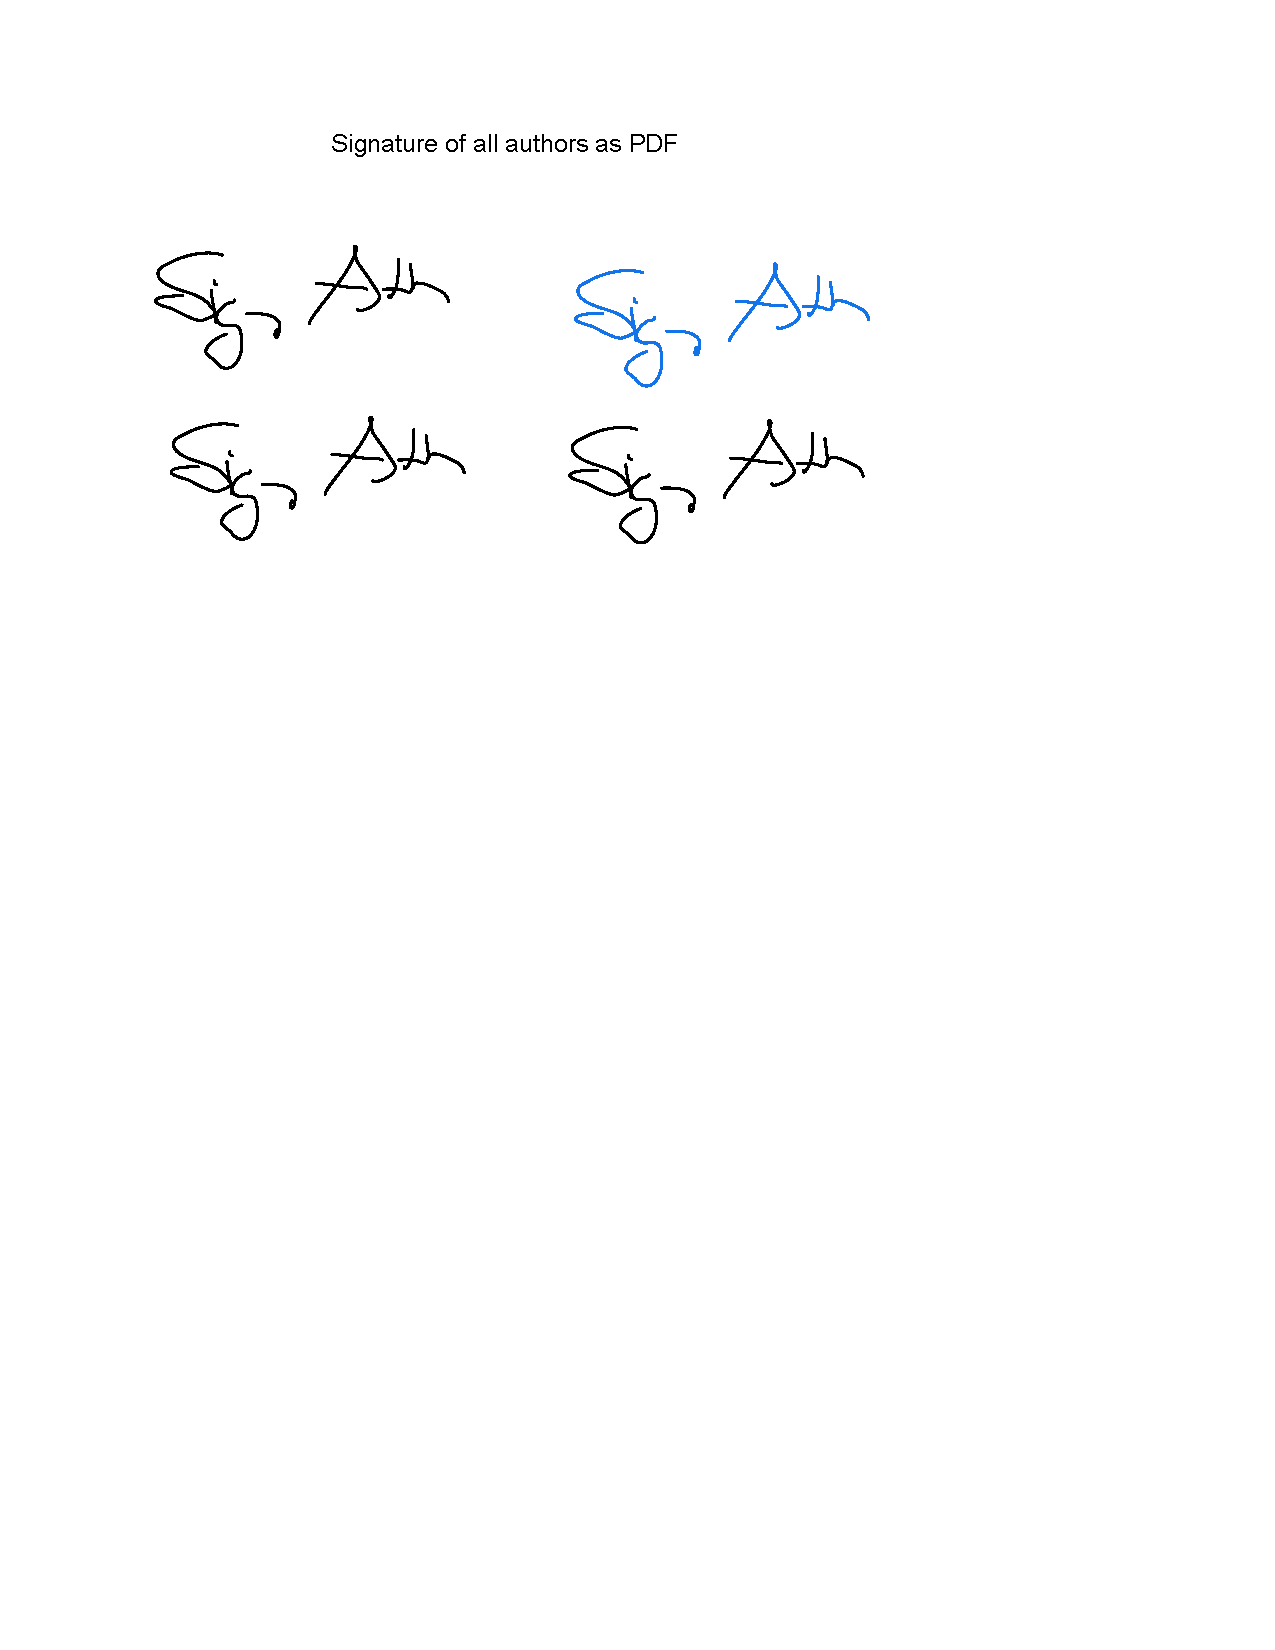
\includegraphics[width=1\textwidth, trim=0pt 500pt 0pt 50pt, clip]{images/example.pdf}
\end{figure}



\end{document}
